\documentclass[12pt]{article}
%%%%%%%%%%%%%%%%%% General pagackages
\usepackage{amssymb,amsmath,amsfonts,eurosym,ulem,graphicx,
	caption,color,setspace,sectsty,comment,footmisc,
	pdflscape,subcaption,array, multicol,multirow,tikz, bm,
        booktabs, rotating, titling}     
%%%%%%%%%%%%%%%%%%% Encoding
\usepackage[utf8]{inputenc}
%%%%%%%%%%%%%%%%%% Margins and Spacing
\usepackage[left=1.0in,right=1.0in,top=1in,bottom=1in]{geometry}
\usepackage{indentfirst}
%%%%%%%%%%%%%%%%%% References
\usepackage[sort]{natbib}
\bibliographystyle{econ}
%%%%%%%%%%%%%%%%%% Links
\usepackage[colorlinks=true, allcolors=blue]{hyperref}
\urlstyle{same} %makes url the same font as text, not courier default
\newcommand{\doi}[1]{\url{#1}}
%%%%%%%%%%%%%%%%%% tikz/diagrams
\usetikzlibrary{arrows,shapes,positioning,intersections,calc}
%%%%%%%%%%%%%%%%%% table formatting
\newcolumntype{L}[1]{>{\raggedright\arraybackslash}p{#1}}
\newcolumntype{C}[1]{>{\centering\arraybackslash}p{#1}}
\newcolumntype{R}[1]{>{\raggedleft\arraybackslash}p{#1}}
\normalem
\makeatother
%%%%%%%%%%%%%%%%%% Autoreference names
\renewcommand{\sectionautorefname}{Section}
\renewcommand{\subsectionautorefname}{Sub-section}
\renewcommand{\figureautorefname}{Figure}
\renewcommand{\tableautorefname}{Table}
\renewcommand{\figureautorefname}{Figure}
% equation numbering start at 1
\newcommand\numberthis{\addtocounter{equation}{1}\tag{\theequation}}
%%%%%%%%%%%%%%%%%% Theorem Names
\newtheorem{prop}{Proposition}
\newtheorem{definition}{Definition}
\newtheorem{lemma}{Lemma}
\newtheorem{corollary}{Corollary}
\newtheorem{result}{Result}
\newtheorem{assumption}{Assumption}
\newtheorem{theorem}{Theorem}

%%%%%%%%%%%%%%%%%% Title Information
%title page single spacing 
\setstretch{1} 
%subtitle command
\newcommand{\subtitle}[1]{\posttitle{\par\end{center}\begin{center}\large#1\end{center}\vskip0.5em}}

\title{[Title: Economics Honors Thesis LaTeX Template]}
\subtitle{Brown University\\Honors Thesis in Economics}
\author{[Name]\thanks{[Acknowledgements and Thanks. This template is based on an example provided by Professor Amy Handlan.]}}
\date{\today}

\begin{document}

\maketitle

\begin{abstract}
    Abstract is a short description of the project.
\end{abstract} 
\doublespacing
\textit{Keywords:} keyword1, keyword2, keyword3
\\
\textit{JEL Codes:} A1 %JEL codes refer to topics of the paper. Assign 3 from https://www.aeaweb.org/econlit/jelCodes.php
% \thispagestyle{empty} 
\newpage
\setstretch{1.75} 
 

\section{Introduction}
In this section, you will introduce you research project, highlight your methods and results, and argue about the broader implications of the project.

\section{Literature Review}
In this section, you will describe the literature related to your research project and your connection to those literatures. To enter a citation in line: \citet{wong2018breakdown}. To enter a citation in parentheses: \citep{CitationExample}. If you enter multiple citations, it will order them alphabetically: \citep{CitationExample,WorkingPaperExample}.

\section{Data}
In this section, you will describe the data sources and variables you use for analysis. You may want to include figures to describe your data. Consider the formatting in \autoref{fig:enter-label}.

\begin{figure}[ht]
    \centering
    \caption{Figure Title}
    \label{fig:enter-label}
    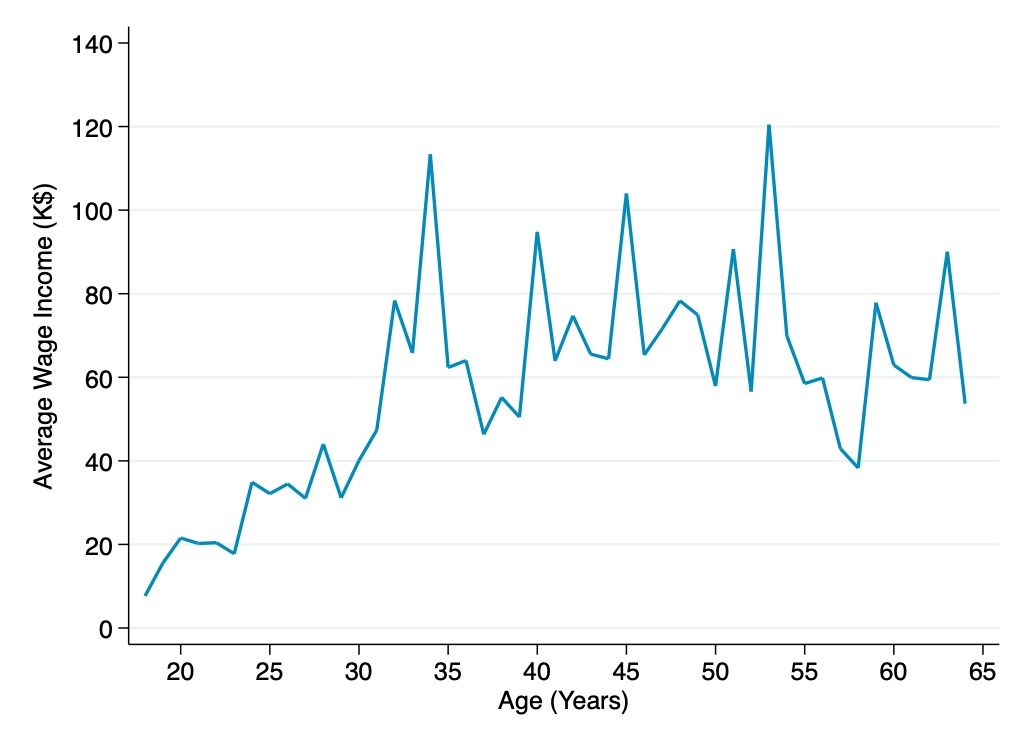
\includegraphics[width=.75\textwidth]{../output/figures/avgwageincome_wage.jpg}
    \caption*{\footnotesize \textit{Note: Describe the figure above.}}
\end{figure}

Additionally, reference \autoref{tab:summarytable} for formatting guidelines for tables:

\begin{table}[ht]
    \centering
    \caption{Summary Table}
    \label{tab:summarytable}
    {
\def\sym#1{\ifmmode^{#1}\else\(^{#1}\)\fi}
\begin{tabular}{l*{1}{ccccc}}
\toprule
                    &        Mean&          SD&         Min&         Max&           N\\
\midrule
Wage income         &      58.734&      71.836&           1&         850&         835\\
Total income        &   63924.501&   79303.953&        1000&      957500&         835\\
Age                 &      40.941&      12.462&          18&          64&         835\\
Female              &       0.497&       0.500&           0&           1&         835\\
White               &       0.734&       0.442&           0&           1&         835\\
Black               &       0.143&       0.350&           0&           1&         835\\
Married             &       0.571&       0.495&           0&           1&         835\\
In labor force      &       1.000&       0.000&           1&           1&         835\\
\bottomrule
\end{tabular}
}

    \caption*{\footnotesize \textit{Note: Describe the table above.}}
\end{table}



\section{Model}
In this section, you will describe the model for your analysis. You can reference equations using the ``equation'' environment or the ``align'' environment. With either you can reference them using labels, as in \autoref{eq:regression} and \autoref{eq:model}.

 In an empirical paper, this will include your research design, assumptions, identification strategy, and regression specification. \autoref{eq:regression} provides a template for writing the regression specification.
\begin{equation}\label{eq:regression}
    y_{s,t} = \alpha +\beta X_{s,t} + \gamma GDP_{s,t} + \sigma POP_{s,t} +\varepsilon_{s,t}
\end{equation}

Where \(X_{s,t}\) is the independent variable measured in state \(s\) and year \(t\), \(GDP_{s,t}\) is a control for yearly state gdp. We will only add the population control \(POP_{s,t}\) in a separate second specification because....

 In theoretical paper, this will include the modeling environment, agents, actions/choices, information sets, and preferences. \autoref{eq:model} provides a template for writing the agent's optimization problem.
\begin{align}\label{eq:model}
    \max_c\ &\ U(c) \\
    \text{s.t.} &\ \ p c \leq e  \nonumber 
\end{align}


\section{Results}

For a regression table, you can look at \autoref{tab:regressiontable}. Python, Stata, and other programs where you will run regression have options to automatically output regression tables to LaTeX format. 

\begin{table}[ht]
    \centering
    \caption{Regression Results}
    \label{tab:regressiontable}
    {
\def\sym#1{\ifmmode^{#1}\else\(^{#1}\)\fi}
\begin{tabular}{l*{4}{c}}
\toprule
                    &\multicolumn{1}{c}{(1)}&\multicolumn{1}{c}{(2)}&\multicolumn{1}{c}{(3)}&\multicolumn{1}{c}{(4)}\\
                    &\multicolumn{1}{c}{Total income}&\multicolumn{1}{c}{Total income}&\multicolumn{1}{c}{Total income}&\multicolumn{1}{c}{Total income}\\
\midrule
Female              &    -22883.7\sym{***}&    -20939.8\sym{***}&    -21827.8\sym{***}&    -18064.1\sym{***}\\
                    &    (4729.3)         &    (4323.2)         &    (4324.8)         &    (4481.8)         \\
\addlinespace
Constant            &     75297.8\sym{***}&     74331.7\sym{***}&     74697.4\sym{***}&     72243.4\sym{***}\\
                    &    (2350.5)         &    (2148.7)         &    (2149.4)         &    (2249.4)         \\
\midrule
Observations        &         835         &         835         &         833         &         787         \\
\(R^{2}\)           &       0.084         &       0.188         &       0.201         &       0.340         \\
State FE            &         Yes         &         Yes         &         Yes         &         Yes         \\
Age FE              &          No         &         Yes         &         Yes         &         Yes         \\
Race FE             &          No         &          No         &         Yes         &         Yes         \\
Industry FE         &          No         &          No         &          No         &         Yes         \\
\bottomrule
\end{tabular}
}

    \caption*{\footnotesize \textit{Note: Describe the table above.}}
\end{table}

Where possible, you should also include results as graphs and figures.

For theoretical model, you results may include theorems. You can format them like \autoref{theorem:example}.
\begin{theorem}[Title of the Theorem]\label{theorem:example}
    Description of the theorem.
\end{theorem}

\section{Conclusion}
In this section, you will conclude the project by summarizing the methods and results. You should also connect back to the introduction, literature, and the big picture.

\newpage
\singlespacing
\bibliography{references_honors}

\end{document}
